\chapter{Implémentation du M2}\label{chap:M2}
\section{Détails de la modélisation}
Construisons un méta-modèle basé sur l'entité \verb+Composant+ :
\begin{itemize}
\item 
  Un \verb+Composant+ possède des \verb+Propriétés+. Ces dernières peuvent être fonctionnelles (\verb+PropFonc+) ou non fonctionnelles (\verb+PropNonFonc+).
\item 
  Il possède deux \verb+InterfaceComposants+ :  une pour les \verb+Services+ requis, une pour les \verb+Services+ fournis.
\item
  Une interface est aussi constituée de \verb+Ports+ (fournis ou requis). 
\item
  Chaque port est associé à un et un seul \verb+Service+, mais un \verb+Service+ possède plusieurs \verb+Ports+.  
\end{itemize}


\paragraph{}
Afin d'effectuer la communication entres composants, il est nécessaire d'introduire la notion de connecteur :

\begin{itemize}
\item 
  Un \verb+Connecteur+ a deux \verb+InterfaceConnecteurs+.
\item
  Chaque \verb+InterfaceConnecteur+ possède deux \verb+Rôles+ : un rôle requis \verb+RoleR+  et un rôle fourni \verb+RoleF+.
\item
  Chaque rôle d'une interface est relié par un lien \verb+attachement+  à son port correspondant (\textit{c.a.d }: un rôle requis à un port requis et un rôle fourni à un port fourni).  
\item
  Les deux interfaces d'un connecteur sont reliés par deux \verb+Glus+, chaque \verb+Glu+  reliant un rôle requis au rôle fournis opposé.
\end{itemize}

\paragraph{}

La \verb+Configuration+  est un composant composé de \verb+Composants+ : 

\begin{itemize}
\item 
  Elle possède deux \verb+InterfaceConfigs+. Ces dernières hériant d'\verb+InterfaceComposant+.
\item
  Il est possible de relier un \verb+PortR+ de l'\verb+InterfaceConfig+ à un \verb+PortR+ d'un composant de la configuration (et réciproquement pour le \verb+PortF+) grâce à un lien \verb+binding+.
\item
  Un connecteur peut être aussi une \verb+Configuration+.
\end{itemize}

\paragraph{Corrections du M2 après évaluation}
Suite aux remarques émises lors de l'évaluation, nous avons apporté les corrections suivantes : 
\begin{enumerate}
\item
  Expliciter un lien direct entre \verb+Connecteur+ et \verb+Glu+.
\item
  Appliquer un pattern \textit{composite} à l'entité \verb+Connecteur+.
\item
  Refactoring de la hiérachie entre \verb+Composant+, \verb+Connecteur+ et \verb+Configuration+. Désormais \verb+Composant+ et \verb+Connecteur+ sont au \og même niveau \fg{} par rapport à \verb+Configuration+.
\end{enumerate}

\section{Diagramme M2}
\pagestyle{empty}
\begin{figure}[htb]
  %\centering
  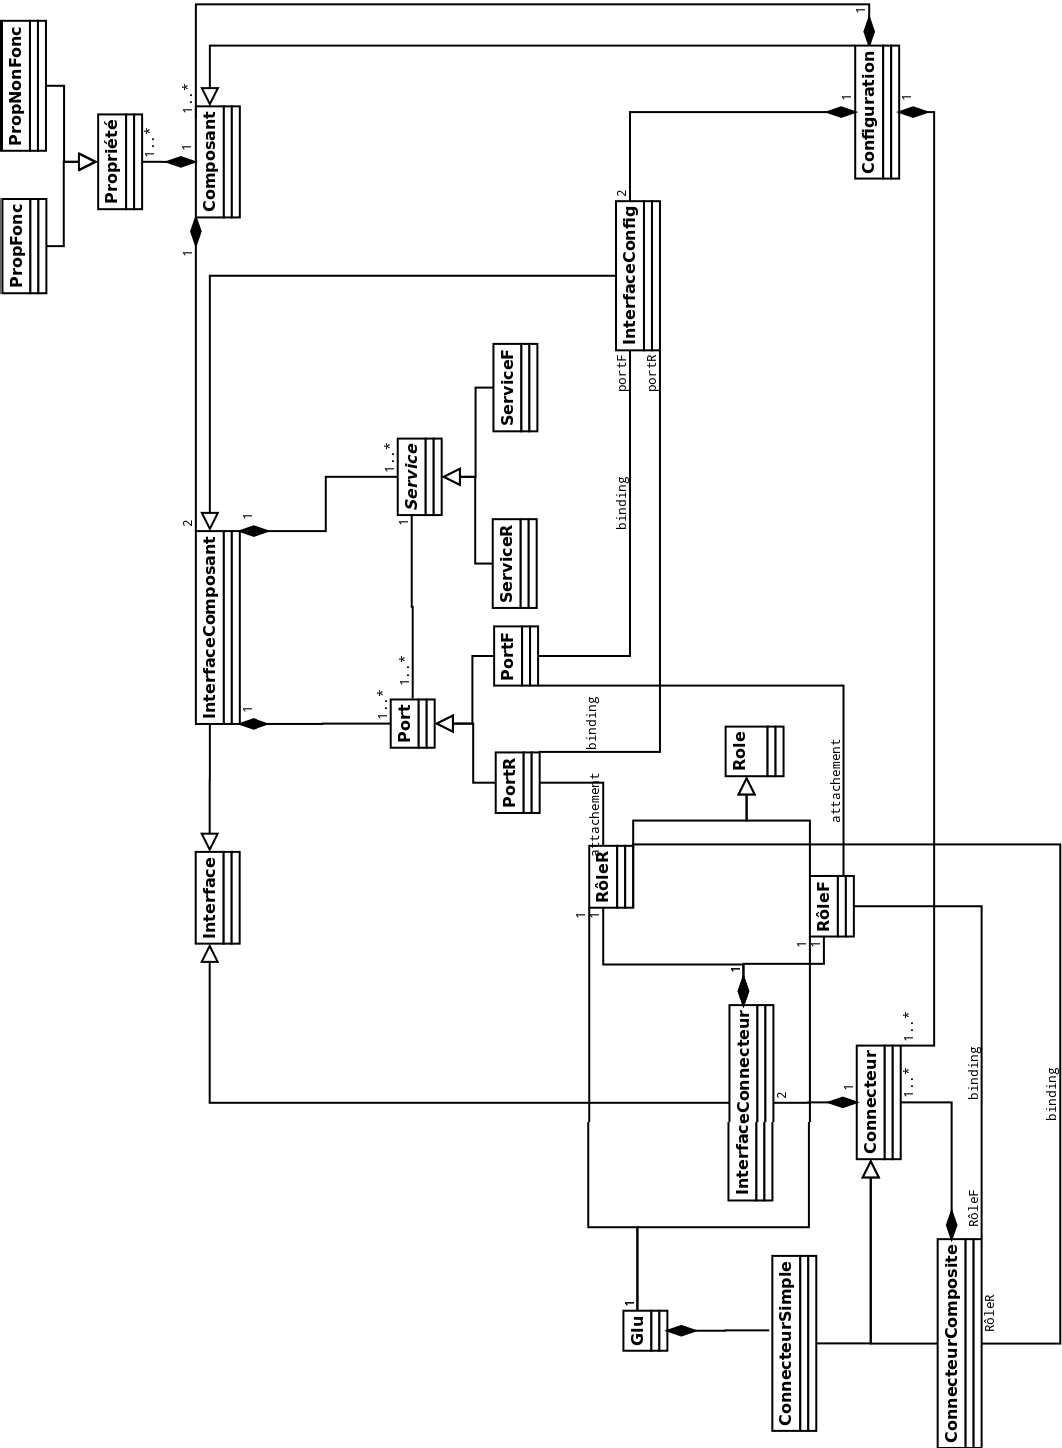
\includegraphics[scale=0.33]{img/M2}
  \caption{Méta-Model (M2)}
  \label{fig:M2}
\end{figure}
